% ============================================================
\chapter{Apprentissage sur les Vari\'et\'es}
\label{ch:varietes}
% ============================================================

Les graphes sont des structures discr\`etes, mais de nombreuses donn\'ees vivent sur des espaces \emph{continus} non euclidiens~: la surface de la Terre, l'espace des rotations 3D, la vari\'et\'e des matrices de covariance. Peut-on d\'efinir des r\'eseaux de neurones directement sur ces \emph{vari\'et\'es diff\'erentiables}~? L'approche g\'eom\'etrique de l'apprentissage profond, syst\'ematis\'ee par Bronstein et al.\ dans leur \og blueprint \fg de 2021, montre que c'est possible --- \`a condition de remplacer les op\'erations euclidiennes (convolution, translation) par leurs analogues riemanniens (transport parall\`ele, application exponentielle). Ce chapitre pose les fondations g\'eom\'etriques n\'ecessaires.

\section{G\'eom\'etrie diff\'erentielle~: rappels}

\subsection{Vari\'et\'es diff\'erentiables}

\begin{definition}[Vari\'et\'e diff\'erentiable]
Une \textbf{vari\'et\'e diff\'erentiable} de dimension $d$ est un espace
topologique $\mathcal{M}$ qui est localement hom\'eomorphe \`a $\R^d$. Plus
pr\'ecis\'ement, pour chaque point $p \in \mathcal{M}$, il existe un voisinage
ouvert $U$ et un hom\'eomorphisme (carte locale) $\varphi: U \to \R^d$. Les
changements de cartes $\varphi_\beta \circ \varphi_\alpha^{-1}$ sont $C^\infty$.
\end{definition}

\begin{exemple}[Vari\'et\'es courantes]
\begin{enumerate}
    \item La \textbf{sph\`ere} $S^2 = \{(x,y,z) \in \R^3 : x^2 + y^2 + z^2 = 1\}$
          --- dimension 2.
    \item Le \textbf{tore} $T^2 = S^1 \times S^1$ --- dimension 2.
    \item Le groupe $\mathrm{SO}(3)$ --- dimension 3.
    \item L'espace des matrices sym\'etriques d\'efinies positives $\mathrm{Sym}^+(n)$.
\end{enumerate}
\end{exemple}

\subsection{Espace tangent et m\'etrique riemannienne}

\begin{definition}[Espace tangent]
L'\textbf{espace tangent} $T_p\mathcal{M}$ en un point $p \in \mathcal{M}$
est l'espace vectoriel des vecteurs tangents \`a $\mathcal{M}$ en $p$. Il
est de dimension $d = \dim(\mathcal{M})$.
\end{definition}

\begin{definition}[M\'etrique riemannienne]
Une \textbf{m\'etrique riemannienne} sur $\mathcal{M}$ est la donn\'ee, pour
chaque $p \in \mathcal{M}$, d'un produit scalaire
$g_p: T_p\mathcal{M} \times T_p\mathcal{M} \to \R$ variant lissement avec $p$.
La paire $(\mathcal{M}, g)$ est une \textbf{vari\'et\'e riemannienne}.
\end{definition}

\begin{formules}[title=\textbf{Objets de base en g\'eom\'etrie riemannienne}]
\begin{itemize}
    \item \textbf{Longueur d'une courbe} $\gamma: [0,1] \to \mathcal{M}$~:
          $L(\gamma) = \int_0^1 \sqrt{g_{\gamma(t)}(\dot{\gamma}(t), \dot{\gamma}(t))}\, dt$
    \item \textbf{Distance g\'eod\'esique}~:
          $d(p, q) = \inf_\gamma L(\gamma)$ sur les courbes reliant $p$ \`a $q$.
    \item \textbf{Application exponentielle}~:
          $\exp_p: T_p\mathcal{M} \to \mathcal{M}$, envoie $v$ sur le point
          atteint par la g\'eod\'esique partant de $p$ dans la direction $v$.
    \item \textbf{Application logarithme}~:
          $\log_p: \mathcal{M} \to T_p\mathcal{M}$, inverse (locale) de $\exp_p$.
\end{itemize}
\end{formules}

\begin{figure}[htbp]
\centering
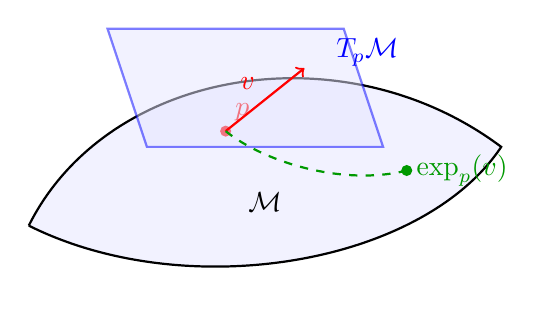
\begin{tikzpicture}
% Variete (surface courbe)
\draw[thick, fill=blue!5] (0,0) .. controls (1,2) and (4,2.5) .. (6,1)
    .. controls (5,-0.5) and (2,-1) .. (0,0);
\node at (3, 0.3) {$\mathcal{M}$};

% Point p
\fill[red] (2.5, 1.2) circle (2pt) node[above right] {$p$};

% Plan tangent
\draw[thick, blue, fill=blue!10, opacity=0.5]
    (1, 2.5) -- (4, 2.5) -- (4.5, 1) -- (1.5, 1) -- cycle;
\node[blue] at (4.3, 2.2) {$T_p\mathcal{M}$};

% Vecteur tangent
\draw[->, thick, red] (2.5, 1.2) -- (3.5, 2) node[midway, above left] {$v$};

% Geodesique
\draw[thick, green!60!black, dashed] (2.5, 1.2) .. controls (3, 0.8) and (4, 0.5) .. (4.8, 0.7);
\fill[green!60!black] (4.8, 0.7) circle (2pt) node[right] {$\exp_p(v)$};
\end{tikzpicture}
\caption{Espace tangent, vecteur tangent et application exponentielle.}
\end{figure}

\section{Op\'erateurs diff\'erentiels sur les vari\'et\'es}

\begin{definition}[Op\'erateur de Laplace--Beltrami]
L'op\'erateur de \textbf{Laplace--Beltrami} est la g\'en\'eralisation du
laplacien \`a une vari\'et\'e riemannienne~:
\[
    \Delta_{\mathcal{M}} f = \mathrm{div}(\mathrm{grad}\, f)
    = \frac{1}{\sqrt{\abs{g}}} \sum_{i,j} \partial_i\!\left(\sqrt{\abs{g}}\,
    g^{ij}\, \partial_j f\right)
\]
o\`u $g^{ij}$ sont les composantes de l'inverse du tenseur m\'etrique et
$\abs{g} = \det(g_{ij})$.
\end{definition}

\begin{theoreme}[Propri\'et\'es de $\Delta_{\mathcal{M}}$]
\begin{enumerate}
    \item $\Delta_{\mathcal{M}}$ est \textbf{auto-adjoint} et \textbf{semi-d\'efini n\'egatif}
          (avec la convention $\Delta f = -\mathrm{div}(\nabla f)$ on a le signe oppos\'e).
    \item Il est \textbf{intrins\`eque}~: ind\'ependant du syst\`eme de coordonn\'ees.
    \item Il g\'en\'eralise le laplacien de graphe~: sur un graphe, $\mathbf{L}$
          est une discr\'etisation de $-\Delta_{\mathcal{M}}$.
    \item Il admet une d\'ecomposition spectrale~:
          $\Delta_{\mathcal{M}} \phi_k = -\lambda_k \phi_k$ avec
          $0 = \lambda_0 \leq \lambda_1 \leq \cdots$
\end{enumerate}
\end{theoreme}

\begin{proposition}[\'Equation de la chaleur sur $\mathcal{M}$]
L'\'equation de la chaleur sur une vari\'et\'e s'\'ecrit~:
\[
    \frac{\partial u}{\partial t} = \Delta_{\mathcal{M}} u
\]
Sa solution est $u(p, t) = \int_{\mathcal{M}} K_t(p, q)\, u_0(q)\, dq$ o\`u
$K_t(p,q) = \sum_k e^{-\lambda_k t} \phi_k(p) \phi_k(q)$ est le
\textbf{noyau de la chaleur}.
\end{proposition}

\section{Convolutions sur les vari\'et\'es}

\subsection{D\'efis}

Sur une vari\'et\'e, la convolution classique pose plusieurs probl\`emes~:
\begin{itemize}
    \item Pas de \textbf{structure de groupe de translation} (sauf pour $\R^n$
          et le tore).
    \item Pas de \textbf{syst\`eme de coordonn\'ees global}.
    \item Le \textbf{transport parall\`ele} est n\'ecessaire pour comparer des
          vecteurs en diff\'erents points.
\end{itemize}

\subsection{Approche spectrale~: MoNet et variantes}

\begin{definition}[MoNet --- Monti et al., 2017]
MoNet (\textit{Mixture Model Networks}) d\'efinit des filtres
param\'etriques dans l'espace des coordonn\'ees locales pseudo-polaires~:
\[
    \mathbf{h}_v^{(\ell+1)} = \sum_{j=1}^{J} \mathbf{W}_j^{(\ell)}
    \sum_{u \in \mathcal{N}(v)} w_j(\mathbf{c}(v, u))\, \mathbf{h}_u^{(\ell)}
\]
o\`u $\mathbf{c}(v, u) = (\rho_{vu}, \theta_{vu})$ sont les coordonn\'ees
pseudo-polaires de $u$ dans le rep\`ere local de $v$, et
$w_j(\mathbf{c}) = \exp\!\left(-\frac{1}{2}(\mathbf{c} - \boldsymbol{\mu}_j)^\top
\boldsymbol{\Sigma}_j^{-1}(\mathbf{c} - \boldsymbol{\mu}_j)\right)$
sont des noyaux gaussiens appris.
\end{definition}

\subsection{Convolution par descripteurs spectraux}

\begin{definition}[Noyau de diffusion]
Le \textbf{noyau de diffusion} d'une vari\'et\'e est d\'efini par~:
\[
    K_t(p, q) = \sum_{k=0}^{\infty} e^{-\lambda_k t}\, \phi_k(p)\, \phi_k(q)
\]
Il d\'efinit un produit scalaire dans un espace de Hilbert \`a noyau reproduisant
(RKHS) et fournit des descripteurs de forme intrins\`eques.
\end{definition}

\begin{definition}[HKS --- Heat Kernel Signature]
Le \textbf{Heat Kernel Signature} est un descripteur intrins\`eque de la
g\'eom\'etrie locale~:
\[
    \mathrm{HKS}(p, t) = K_t(p, p) = \sum_{k=0}^{\infty} e^{-\lambda_k t}\, \phi_k(p)^2
\]
Il encode l'information multi-\'echelle~: petits $t$ capturent la g\'eom\'etrie
locale, grands $t$ la g\'eom\'etrie globale.
\end{definition}

\begin{codeblock}[title=\textbf{Calcul du HKS sur un maillage}]
\begin{minted}{python}
import torch
import numpy as np

def compute_hks(eigenvalues, eigenvectors, time_scales):
    """Calcul du Heat Kernel Signature.

    Args:
        eigenvalues: (K,) valeurs propres du laplacien
        eigenvectors: (N, K) vecteurs propres
        time_scales: (T,) echelles de temps
    Returns:
        hks: (N, T) descripteurs HKS
    """
    # eigenvalues: (K,), eigenvectors: (N, K), time_scales: (T,)
    # exp(-lambda_k * t): (K, T)
    exp_vals = torch.exp(
        -eigenvalues.unsqueeze(1) * time_scales.unsqueeze(0)
    )
    # phi_k(p)^2: (N, K)
    phi_sq = eigenvectors ** 2
    # HKS(p, t) = sum_k exp(-lambda_k * t) * phi_k(p)^2
    hks = phi_sq @ exp_vals  # (N, T)
    return hks

# Exemple avec 100 valeurs propres et 16 echelles
eigenvalues = torch.linspace(0, 10, 100)
eigenvectors = torch.randn(500, 100)  # 500 sommets
eigenvectors, _ = torch.linalg.qr(eigenvectors)
time_scales = torch.logspace(-2, 2, 16)

hks = compute_hks(eigenvalues, eigenvectors[:, :100], time_scales)
print(f"Descripteurs HKS: {hks.shape}")  # (500, 16)
\end{minted}
\end{codeblock}

\section{Convolution par transport parall\`ele}

\begin{definition}[Transport parall\`ele]
Le \textbf{transport parall\`ele} le long d'une courbe $\gamma: [0,1] \to \mathcal{M}$
est une application lin\'eaire $\Gamma_\gamma: T_{\gamma(0)}\mathcal{M} \to
T_{\gamma(1)}\mathcal{M}$ qui transporte un vecteur tangent le long de $\gamma$
en pr\'eservant le produit scalaire et en satisfaisant l'\'equation~:
\[
    \nabla_{\dot{\gamma}} V = 0
\]
o\`u $\nabla$ est la connexion de Levi-Civita.
\end{definition}

\begin{definition}[Gauge Equivariant CNN --- de Haan et al., 2021]
Un \textbf{Gauge Equivariant CNN} d\'efinit des convolutions sur une vari\'et\'e
en utilisant des \textbf{rep\`eres locaux} (gauges) et le transport parall\`ele~:
\[
    [f * \psi](p) = \int_{\mathcal{M}} f(\Gamma_{q \to p}\, \cdot)\,
    \psi(\exp_p^{-1}(q))\, dq
\]
Le r\'eseau est \'equivariant par changement de jauge~: le choix du rep\`ere local
n'affecte pas la sortie.
\end{definition}

\section{Apprentissage sur des vari\'et\'es sp\'ecifiques}

\subsection{Convolutions sur la sph\`ere}

\begin{definition}[Spherical CNN --- Cohen et al., 2018]
Les \textbf{Spherical CNNs} d\'efinissent des convolutions sur $S^2$ en
utilisant les harmoniques sph\'eriques comme base spectrale~:
\[
    [f * \psi](\hat{\mathbf{r}}) = \sum_{\ell=0}^{L} \sum_{m=-\ell}^{\ell}
    \hat{f}_\ell^m\, \hat{\psi}_\ell\, Y_\ell^m(\hat{\mathbf{r}})
\]
o\`u $\hat{f}_\ell^m$ et $\hat{\psi}_\ell$ sont les coefficients dans la base
des harmoniques sph\'eriques. Pour un filtre \textbf{zonal}
(invariant par rotation autour de l'axe), $\hat{\psi}_\ell$ ne d\'epend que
de $\ell$.
\end{definition}

\begin{theoreme}[\'Equivariance par $\mathrm{SO}(3)$]
La convolution sph\'erique est \'equivariante par rotation~: si
$R \in \mathrm{SO}(3)$ et $L_R f(\hat{\mathbf{r}}) = f(R^{-1}\hat{\mathbf{r}})$, alors~:
\[
    L_R(f * \psi) = (L_R f) * \psi
\]
\end{theoreme}

\subsection{Apprentissage sur les groupes de Lie}

\begin{definition}[LieConv --- Finzi et al., 2020]
LieConv d\'efinit des convolutions directement sur les groupes de Lie en
utilisant un \textbf{noyau continu} param\'etr\'e dans l'alg\`ebre de Lie~:
\[
    [f * \psi](g) = \int_G f(h)\, \psi(\log(h^{-1}g))\, d\mu(h)
\]
En pratique, l'int\'egrale est approch\'ee par Monte Carlo sur un voisinage
\'echantillonn\'e.
\end{definition}

\section{Applications~: analyse de formes 3D}

\begin{definition}[Correspondance de formes]
Le probl\`eme de \textbf{correspondance de formes} consiste \`a trouver une
application $T: \mathcal{M}_1 \to \mathcal{M}_2$ entre deux surfaces qui
pr\'eserve la structure g\'eom\'etrique. Les m\'ethodes spectrales utilisent
les \textbf{cartes fonctionnelles}~:
\[
    \mathbf{C} = \boldsymbol{\Phi}_2^\dagger\, T_f\, \boldsymbol{\Phi}_1
\]
o\`u $\boldsymbol{\Phi}_i$ sont les matrices des fonctions propres du laplacien
tronqu\'e et $T_f$ est l'op\'erateur de correspondance fonctionnelle.
\end{definition}

\begin{codeblock}[title=\textbf{Cartes fonctionnelles pour la correspondance de formes}]
\begin{minted}{python}
import torch

def functional_map(phi_1, phi_2, descriptors_1, descriptors_2, k=30):
    """Calcul d'une carte fonctionnelle.

    Args:
        phi_1, phi_2: (N, k) fonctions propres tronquees
        descriptors_1, descriptors_2: (N, d) descripteurs (HKS, etc.)
        k: nombre de fonctions propres
    Returns:
        C: (k, k) matrice de carte fonctionnelle
    """
    # Projection des descripteurs dans la base spectrale
    A1 = phi_1[:, :k].T @ descriptors_1  # (k, d)
    A2 = phi_2[:, :k].T @ descriptors_2  # (k, d)

    # Resolution au sens des moindres carres : C * A1 = A2
    C, _ = torch.linalg.lstsq(A1.T, A2.T)
    C = C.T  # (k, k)
    return C

# Exemple
N = 1000  # nombre de sommets
k = 30    # taille de la base
phi_1 = torch.randn(N, k)
phi_2 = torch.randn(N, k)
desc_1 = torch.randn(N, 16)
desc_2 = torch.randn(N, 16)
C = functional_map(phi_1, phi_2, desc_1, desc_2, k=k)
print(f"Carte fonctionnelle: {C.shape}")  # (30, 30)
\end{minted}
\end{codeblock}

\section{Optimisation sur les vari\'et\'es}

\begin{definition}[Gradient riemannien]
Le \textbf{gradient riemannien} d'une fonction $f: \mathcal{M} \to \R$ en $p$
est l'unique vecteur $\mathrm{grad}\, f(p) \in T_p\mathcal{M}$ tel que~:
\[
    g_p(\mathrm{grad}\, f(p), v) = df_p(v), \quad \forall v \in T_p\mathcal{M}
\]
\end{definition}

\begin{algorithme}[title=\textbf{Descente de gradient riemannienne}]
\begin{enumerate}
    \item Calculer le gradient euclidien $\nabla f(\mathbf{x})$.
    \item Projeter sur l'espace tangent~: $\xi = \mathrm{Proj}_{T_\mathbf{x}\mathcal{M}}(\nabla f)$.
    \item Effectuer un pas de r\'etraction~: $\mathbf{x}' = \mathrm{Retr}_\mathbf{x}(-\eta\, \xi)$.
\end{enumerate}
Pour $\mathrm{SO}(n)$, la r\'etraction est $\mathrm{Retr}_Q(\xi) = \mathrm{qr}(Q + \xi)$.
\end{algorithme}

\begin{codeblock}[title=\textbf{Optimisation sur la sph\`ere avec geoopt}]
\begin{minted}{python}
import torch
import geoopt

# Variable sur la sphere S^{n-1}
sphere = geoopt.Sphere()
x = sphere.random(torch.Size([10]), dtype=torch.float)
x = geoopt.ManifoldParameter(x, manifold=sphere)

# Fonction objectif : minimiser la distance a un point cible
target = sphere.random(torch.Size([10]), dtype=torch.float)
optimizer = geoopt.optim.RiemannianAdam([x], lr=0.01)

for step in range(100):
    optimizer.zero_grad()
    loss = (x - target).norm() ** 2
    loss.backward()
    optimizer.step()

print(f"Distance finale: {(x - target).norm():.6f}")
print(f"Sur la sphere: {x.norm():.6f}")  # doit etre ~1
\end{minted}
\end{codeblock}

\section*{Exercices}

\begin{exercice}[Laplace--Beltrami sur la sph\`ere]
\begin{enumerate}
    \item Montrer que les harmoniques sph\'eriques $Y_\ell^m$ sont fonctions
          propres de $\Delta_{S^2}$ avec valeurs propres $\lambda_\ell = \ell(\ell+1)$.
    \item Calculer les premi\`eres harmoniques sph\'eriques et les visualiser.
\end{enumerate}
\end{exercice}

\begin{exercice}[Noyau de la chaleur]
\begin{enumerate}
    \item Calculer analytiquement le noyau de la chaleur sur le cercle $S^1$.
    \item Impl\'ementer le calcul num\'erique du noyau de la chaleur sur un
          maillage triangulaire.
    \item Visualiser la diffusion de la chaleur \`a diff\'erentes \'echelles $t$.
\end{enumerate}
\end{exercice}

\begin{exercice}[Transport parall\`ele]
\begin{enumerate}
    \item Calculer le transport parall\`ele le long d'un m\'eridien de la sph\`ere.
    \item Montrer que le transport parall\`ele autour d'un triangle sph\'erique
          induit une rotation d'angle \'egal \`a l'exc\`es sph\'erique.
    \item Impl\'ementer le transport parall\`ele discret sur un maillage.
\end{enumerate}
\end{exercice}

\begin{exercice}[Correspondance de formes]
Impl\'ementer un pipeline de correspondance de formes utilisant~:
\begin{enumerate}
    \item Les descripteurs HKS comme attributs de n\oe uds.
    \item Un GNN pour apprendre des descripteurs \'equivariants.
    \item Les cartes fonctionnelles pour la correspondance.
\end{enumerate}
\end{exercice}
